\hypertarget{pehelpers_8h}{\section{Dokumentacja pliku core/file\-\_\-types/pehelpers.h}
\label{pehelpers_8h}\index{core/file\-\_\-types/pehelpers.\-h@{core/file\-\_\-types/pehelpers.\-h}}
}
{\ttfamily \#include $<$Q\-List$>$}\\*
{\ttfamily \#include $<$Q\-Map$>$}\\*
{\ttfamily \#include $<$Q\-String$>$}\\*
{\ttfamily \#include $<$Q\-Process$>$}\\*
{\ttfamily \#include $<$Q\-File$>$}\\*
{\ttfamily \#include $<$Q\-File\-Info$>$}\\*
{\ttfamily \#include $<$Q\-Dir$>$}\\*
Wykres zależności załączania dla pehelpers.\-h\-:
\nopagebreak
\begin{figure}[H]
\begin{center}
\leavevmode
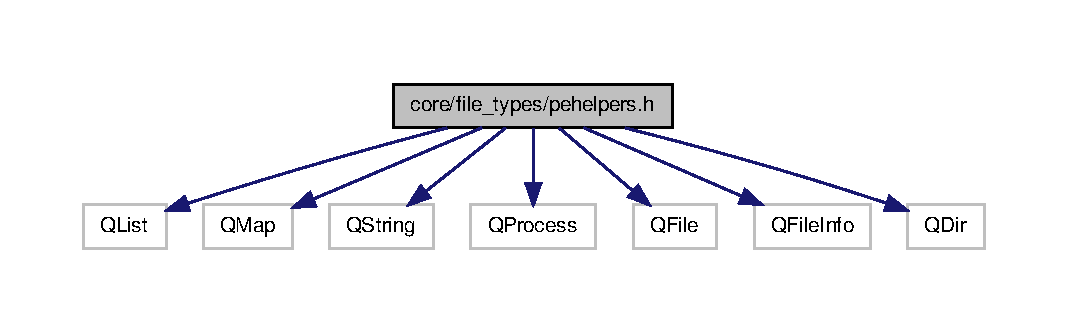
\includegraphics[width=350pt]{pehelpers_8h__incl}
\end{center}
\end{figure}
Ten wykres pokazuje, które pliki bezpośrednio lub pośrednio załączają ten plik\-:
\nopagebreak
\begin{figure}[H]
\begin{center}
\leavevmode
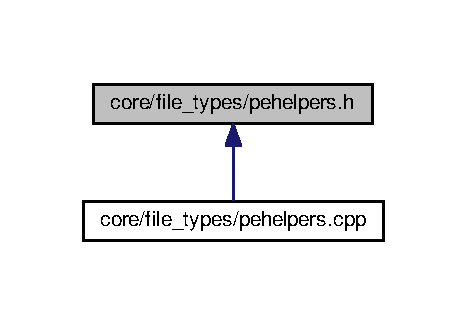
\includegraphics[width=224pt]{pehelpers_8h__dep__incl}
\end{center}
\end{figure}
